\begin{center}
\section{Mini-Project: Create obstacle Resistance Robot, given obstacle should be created by user}
%\addcontentsline{toc}{section}{\protect\numberline{}Search fixed target using the ultrasonic Sensor.}%
\end{center}
\label{sec:first-n-follow}

\subsection{Introduction}
%\addcontentsline{toc}{subsection}{\protect\numberline{Introduction}}%
In the realm of robotics, the ability of a robot to navigate and adapt to its surroundings is crucial for various applications. The evolution of robotic technology has paved the way for the creation of robots that possess the capability to interact with obstacles intelligently. In this project, we delve into the exciting realm of creating an obstacle-resistant robot, where the user becomes the architect of challenges.

Traditionally, robots have been designed to carry out predefined tasks with limited autonomy. However, the concept of obstacle resistance pushes the boundaries of robotics, allowing the robot to dynamically respond to the environment it encounters. This project empowers users to construct obstacles that the robot will encounter, triggering responsive behaviors based on the robot's interactions with these barriers.

Through the integration of sensors into the robot's framework, we open the door to a new dimension of robotic interaction. These sensors, meticulously placed and added to the robot using the `addPart()` method, provide a tangible connection between the robot and its environment. We introduce touch sensors that can sense pressure changes and light sensors that detect intensity levels, thus enabling the robot to perceive and navigate its surroundings.

By simulating a scenario where obstacles are introduced into the robot's path, we explore how the robot's behavior adapts and evolves in response. The dynamic interaction between the robot and the obstacles emphasizes the importance of real-time decision-making and demonstrates the potential for robots to seamlessly integrate into unpredictable environments.

Through the utilization of the `ch.aplu.robotsim` library, we emulate these scenarios with precision and accuracy. As the robot encounters the user-defined obstacles, it responds by reversing its motion and altering its direction, showcasing the potential of intelligent obstacle resistance.

As we proceed with this project, we gain insights into the fascinating world of robotic sensors, user-defined challenges, and the intricate dance between technology and environment. This endeavor not only nurtures innovation in robotics but also brings forth a deeper understanding of the symbiotic relationship between robots and their surroundings.


\subsection{Methodology}
%\addcontentsline{toc}{subsection}{\protect\numberline{Methodology}}
The provided Java code implements an \textit{Obstacle Resistance Robot} using the \texttt{ch.aplu.robotsim} library. This robot is designed to navigate an environment containing user-defined obstacles. The goal is to create a robot that can autonomously navigate around obstacles it encounters.

\subsection{Importing Libraries and Defining Obstacles}

The code starts by importing the necessary libraries from \texttt{ch.aplu.robotsim}. It utilizes the \texttt{RobotContext} class to define obstacles within the simulation environment. Obstacles are added using the \texttt{useObstacle} method, which specifies the obstacle's sprite image and its position (x, y) on the simulation grid.

\subsection{Robot Initialization and Components}

The \texttt{ObstacleRes} class is defined, which contains the robot's behavior. A Lego robot is created using the \texttt{LegoRobot} class. The robot is equipped with a \texttt{Gear} component for movement and a \texttt{TouchSensor} component to detect obstacles.

\subsection{Robot Behavior}

The robot's gear is set to a speed of 30 and is set in forward motion. The code enters an infinite loop where the robot constantly checks the state of the touch sensor. If the touch sensor is pressed (indicating an obstacle collision), the robot responds by performing the following actions:
\begin{enumerate}
    \item Move backward for a duration of 1200 milliseconds to clear the obstacle.
    \item Turn left for a duration of 750 milliseconds to change direction.
    \item Resume forward motion.
\end{enumerate}

\subsection{Main Execution}

In the \texttt{main} method, an instance of the \texttt{ObstacleRes} class is created, initiating the behavior of the obstacle resistance robot.



    
\subsection{Code}
%\addcontentsline{toc}{subsection}{\protect\numberline{Code}}%

\label{subsec:code-first-n-follow}
\href{https://github.com/Mithunprb/MSc-Practicals-Journals/tree/main/MSc-Part2/Robotics/Mini-Project/src}{https://github.com/Mithunprb/MSc-Practicals-Journals/tree/main/MSc-Part2/Robotics/Mini-Project/src}  \\

\begin{minted}[mathescape, linenos, bgcolor=bg, frame=lines, framesep=2mm]{java}
/*
Create obstacle Resistance Robot, given obstacle should be created by user.
 */
package obstacleres;
import ch.aplu.robotsim.*;

public class ObstacleRes
{
  static
  {
    RobotContext.showNavigationBar();
    RobotContext.useObstacle("sprites/bar0.gif", 250, 150);
    RobotContext.useObstacle("sprites/bar1.gif", 400, 250);
    RobotContext.useObstacle("sprites/torch.png", 250, 275);
    RobotContext.useObstacle("sprites/bar2.gif", 250, 400);
    RobotContext.useObstacle("sprites/bar3.gif", 100, 250);
  }

  public ObstacleRes()
  {
    LegoRobot robot = new LegoRobot();
    Gear gear = new Gear();
    TouchSensor ts = new TouchSensor(SensorPort.S3);
    robot.addPart(gear);
    robot.addPart(ts);
    gear.setSpeed(30);
    gear.forward();
    while (true)
    {
      if (ts.isPressed())
      {
        gear.backward(1200);
        gear.left(750);
        gear.forward();
      }
    }
  }

  public static void main(String[] args)
  {
    new ObstacleRes();
  }
}
\end{minted}
\newpage
\subsection{Result}
%\addcontentsline{toc}{subsection}{\protect\numberline{Result}}%


\begin{figure}[h]
  \centering
  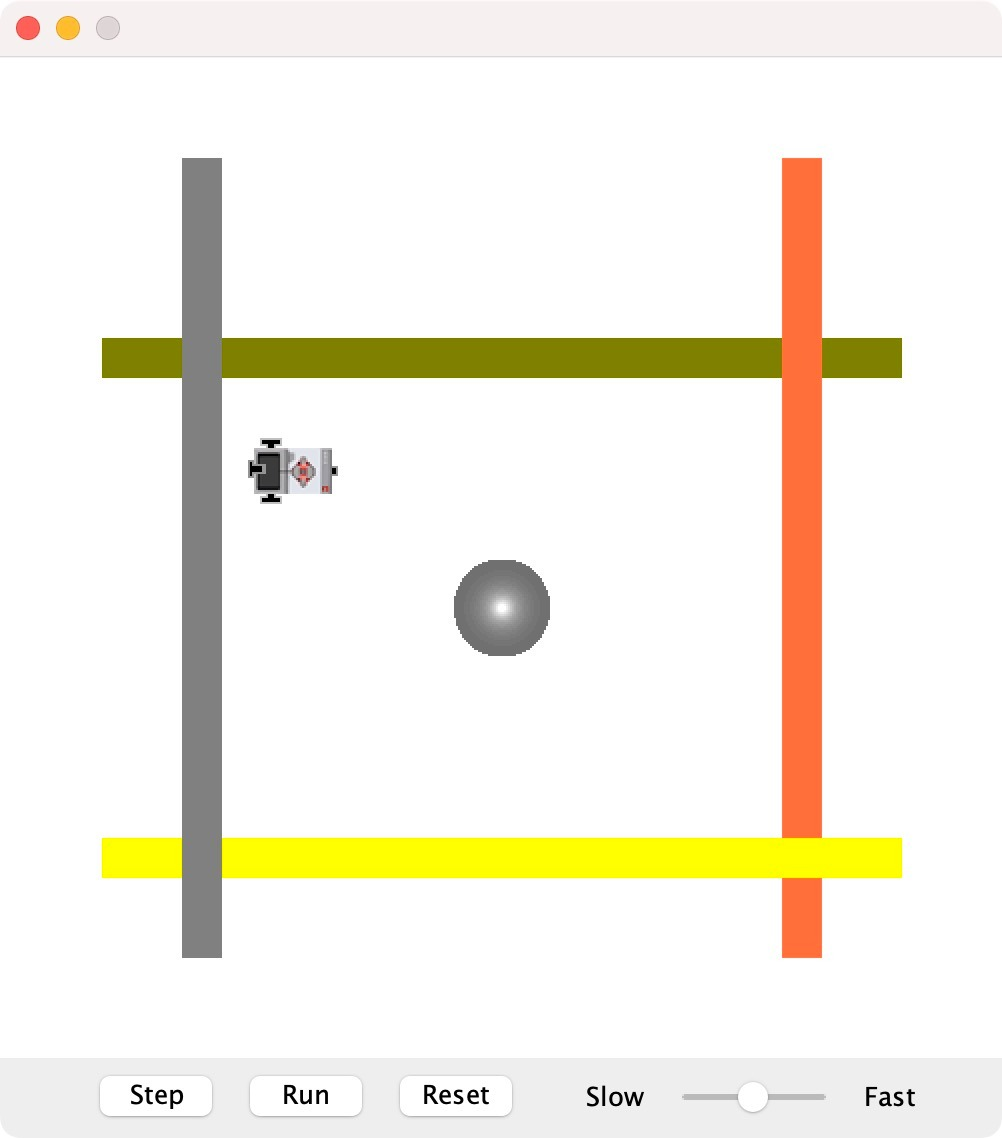
\includegraphics[width=0.5\textwidth]{images/result.jpeg}
  \caption{Simulation Result}
  \label{fig:result}
\end{figure}



\subsection{Conclusion}
%\addcontentsline{toc}{subsection}{\protect\numberline{Conclusion}}%
In the realm of robotics, the development of an obstacle-resistant robot presents an exciting fusion of technology and user engagement. This project has delved into the intricate world of robotic sensors, allowing the robot to dynamically respond to obstacles, a feat previously reserved for advanced artificial intelligence.

By harnessing the power of sensors, our robot has demonstrated its ability to sense and interact with its environment in a meaningful way. The integration of touch sensors that detect physical contact and light sensors that gauge intensity levels has elevated the robot's interaction beyond mere navigation. It has endowed the robot with the ability to perceive its surroundings and make decisions based on real-time feedback, mirroring the adaptability of living organisms.

User participation becomes a cornerstone of this project, blurring the lines between creator and creation. By allowing users to construct obstacles that the robot encounters, we highlight the versatility of robotics in responding to a multitude of scenarios. This bridges the gap between theoretical knowledge and practical implementation, fostering a deeper understanding of robotics among enthusiasts and learners.

The `ch.aplu.robotsim` library has proven to be an invaluable tool in simulating and testing these interactions. Through the simulation, we have observed how the robot's behavior evolves as it faces varying obstacles. The ability to visualize and iterate upon scenarios in a controlled environment empowers us to fine-tune the robot's responsiveness and decision-making capabilities.

The creation of an obstacle-resistant robot goes beyond the realms of technology. It intertwines innovation with user engagement, redefining how we perceive and interact with robots. As robotics continues to advance, projects like these exemplify the potential of machines not just as tools, but as adaptable companions in our ever-changing world. This exploration marks the beginning of an exciting journey toward more intelligent and context-aware robotic systems.